\section{Introduction}
\label{sec:intro}

Google has predicted flu outbreaks by analyzing social network information a
week faster than CDC~\cite{googleflu}. Analysis of twitter data can reveal social
upheavals faster than journalists. Amazon is planning to use customer data for
preemptive shipping of products. Real-time analysis of personal genome may
significantly aid in diagnostics. Big Data analytics are potentially going to
have revolutionary impact on the way scientific discoveries are made. By many
accounts, complex analysis of Big Data is going to be the biggest economic
driver for the IT industry.

Big Data by definition doesn’t fit in personal computers or DRAM of even
moderate size clusters. Since the data may be stored on hard disks, latency and
throughput of storage access is of primary concern. Historically, this has been
mitigated by organizing the processing of data in a highly sequential manner.
However, complex queries cannot always be organized for sequential data
accesses, and thus high performance implementations of such queries pose a
great challenge. One approach to solving this problem is \emph{ram
cloud}~\cite{ramcloud}, where the cluster has enough collective DRAM to accommodate the
entire dataset in DRAM. In this paper, we explore much cheaper alternatives
where Big Data analytics can be done with reasonable efficiency in a single
rack.

Another alternative to speed up complex data analysis is to use SSDs instead of
disks because of superior performance of flash devices in terms of latency of
access and throughput, especially for random accesses. SSDs have been developed
with the goal to be a drop-in replacement of hard disks. This has led to their
widespread use especially in embedded space, but the use of this legacy
interface has resulted in suboptimal use of flash capabilities. The
sub-optimality arises both from the use of a \emph{Flash Translation Layer}
(FTL), and the use of old hardware interfaces like SATA. The latter is somewhat
mitigated by the use of newer interfaces like PCIe.  High-performance enterprise
SSDs such as FusionIO~\cite{fusionio}, Violinmemory~\cite{violinmemory} and Intel NVMe
devices~\cite{intelnvme} solve many of these issues by implementing an improved interface
such as NVMe over PCIe. Attempts to remove the FTL and let the database make
high level decisions~\cite{noftl} have shown to be beneficial, but such
solutions are not yet widely adopted.


The latency to access storage over Ethernet in a hard-disk-based cluster is
dominated by the latency of the hard disk itself. However, this is not the case
in an SSD-based cluster, where network latency may even be larger than the SSD
latency. At this low-level of latency, even software stack overhead becomes a
significant concern. These concerns have been addressed by faster network
fabrics such as 10Gb Ethernet and Infiniband~\cite{infiniband}, and by low-overhead
software protocols such as RDMA~\cite{rdmampi} or user-level TCP stacks that bypass the
operating system~\cite{usertcp}. QuickSAN integrates a network interface into the
storage device, thus removing a layer of software overhead.

Another solution to the network performance problem is to reduce the network
traffic by in-store computing. For example, if one can perform some filtering
operation in the disk controller without bringing it to the host, it may
dramatically reduce the amount of data that needs to be transferred between the
disk and the host~\cite{idisk,netezza,smartssdquery}. Even though this idea has been
around for a long time, it has not found much traction, perhaps because the
characteristics of disks masked the benefits of this approach.  

In this paper, we present FlashBoost, a system designed to address all of the
aforementioned problems in the context of complex analysis of Big Data. Our goal
is to provide a rack-level system which can address many Big Data problems whose
datasets are 10\textasciitilde20 TB. Specifically, we have implemented a system which has 20
nodes where each node consists of a server with 12 Xeon cores, 48 GB of DRAM and
2 TB of disk. We have augmented each server with a Xilinx VC707 FPGA board and
1TB of flash on a custom design board. The FPGA board is connected to the server
via PCIe on one side, and to the flash card by 8 lanes of 6.6Gbps serial
communication links. All FPGAs can be connected to each other in various
topologies using 8 10Gbps serial links provided by the FPGA. The overall
architecture can be seen in Figure~\ref{fig:architecture}.

The system hardware and software provides the following capabilities:
\begin{enumerate}
\item Large enough storage to host Big Data workloads in the 10\textasciitilde20 TB range
\item Near-uniform latency access into a network of storage devices that form a
global address space
\item Capacity to implement user-defined in-storage processing engines in the
embedded FPGA
\item Flash card design which exposes a low-latency interface with details to
exploit parallelism in flash chip accesses by in-storage processing engines
\end{enumerate}

Our preliminary experimental results show that FlashBoost performance is
significantly better than (1) a disk-based system and (2) a flash-based system
in which flash is used as a disk replacement. We also show that accelerators can
provide a factor of XXX performance benefits over a non-accelerated system.
FlashBoost unambiguously establishes an architecture whose
price-performance-power characteristics provide an attractive alternative for
doing similar scale applications in a ram cloud.

The main contributions of this work are: (1) Design and implementation of a
scalable flash-based system with a global address space and in-store computing
capability. (2) A hardware-software codesign environment for incorporating
user-defined in-store processing engines. (3) Performance measurements that show
the advantage of such an architecture over using flash as a drop-in replacement
for disks. (4) Demonstration of a complex data analytics appliance which is much
cheaper and consumes an order of magnitude less power than the cloud-based
alternative.

The rest of the paper is organized as follows: In section~\ref{sec:related} we
explore some existing research related to our system. In
section~\ref{sec:architecture} we describe the architecture of our rack-level
system, and in section~\ref{sec:software} we describe the software interface
that can be used to access flash and the accelerators. In
section~\ref{sec:acceleration} we describe some example accelerators we have
built for the FlashBoost system. In section~\ref{sec:implementation} we describe
our hardware implementation of FlashBoost, and show our results from the
implementation in section~\ref{sec:results} and \ref{sec:results_acceleration}.

\begin{figure*}[ht]
	\begin{center}
	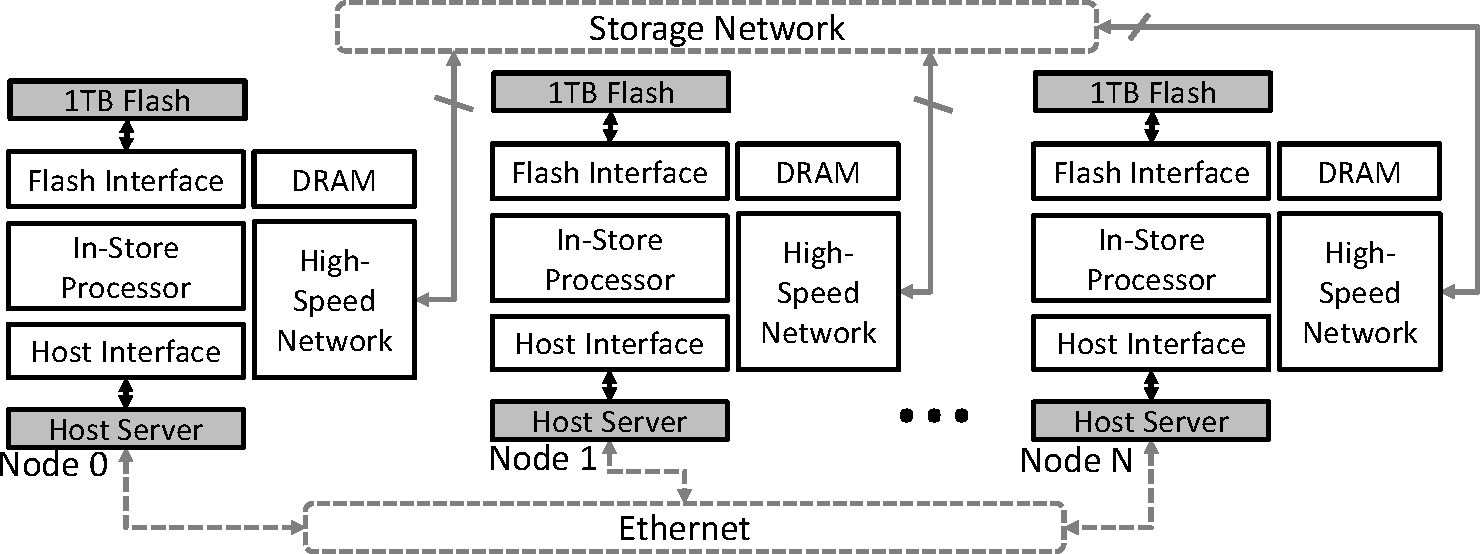
\includegraphics[width=0.8\paperwidth]{figures/architecture-crop.pdf}
	\caption{FlashBoost Architecture}
	\label{fig:architecture}
	\end{center}
\end{figure*}

